\section{SatNOGS-Netzwerk}
\label{sec:sat}
Das SatNOGS-Netzwerk spielt eine zentrale Rolle in unserer Diplomarbeit und bietet hunderten Forschern, Amateurfunkern und Interessierten eine Plattform für verlässliche Kommunikation mit Satelliten.\\

Das, was SatNOGS zu so einer attraktiven Lösung macht, ist der Fakt dass die Bodenstationen um den ganzen Globus verteilt sind. Der große Vorteil davon ist, dass der Empfang von Satellitendaten nun über alle verfügbaren Empfangsstationen laufen kann.\\

In Abbildung \ref{fig:SatNOGS_Erklärung} wird die Topologie des SatNOGS-Netzwerkes abstrahiert dargestellt.
Alle über das Netzwerk verfügbaren Bodenstationen sind mit SatNOGS-Servern verbunden. Auf diese Server kann über die Website bzw. API zugegriffen werden, welche die empfangenen Satellitendaten für alle Benutzer erreichbar macht.

\begin{figure}[h!]
	\centering
	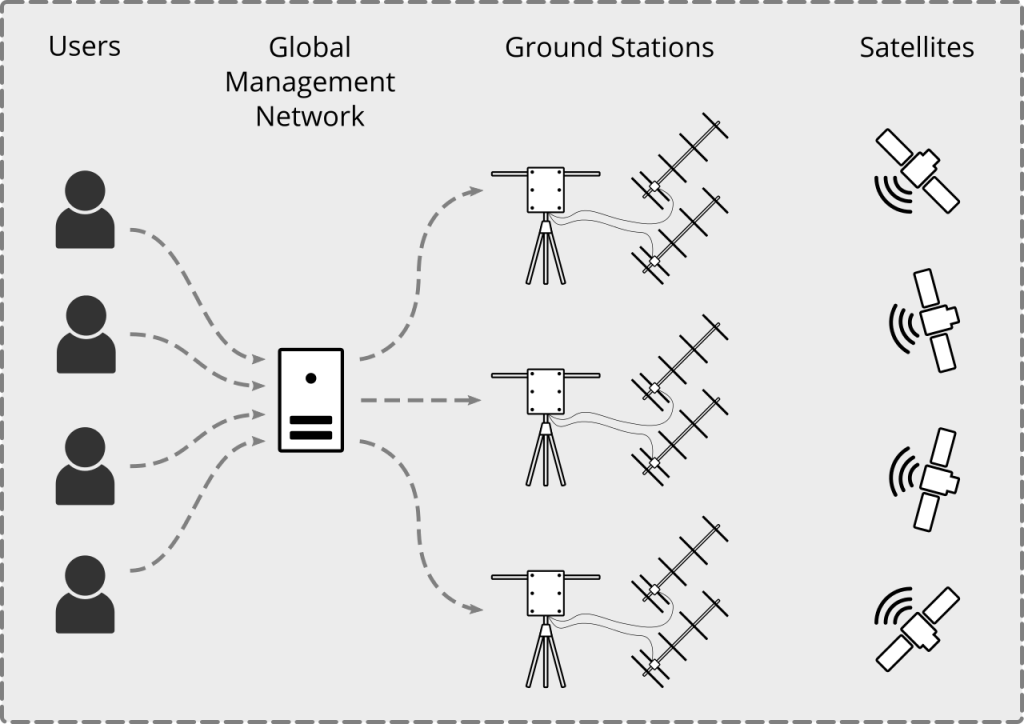
\includegraphics[width=\textwidth]{../ref/SatNOGS_explanation}
	\caption{Erklärung des SatNOGS Netzwerkes}
	\label{fig:SatNOGS_Erklärung}
\end{figure}	

\begin{figure}[h!]
	\centering
	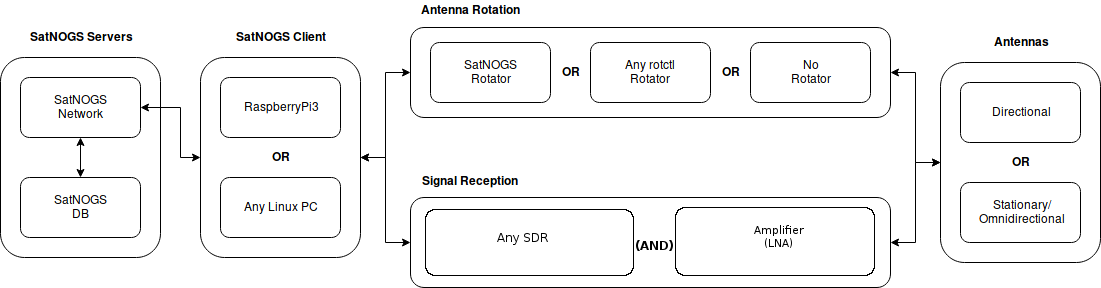
\includegraphics[width=\textwidth]{../ref/SatNOGS_BlockDiagram}
	\caption{SatNOGS-Systemtopologie}
	\label{fig:SatNOGS_Systemtopologie}
\end{figure}

Um näher auf den Ablauf des Datenempfangs und der benötigten Systemblöcke einzugehen wird auf Abbildung \ref{fig:SatNOGS_Systemtopologie} verwiesen.\\

Für den Empfang von Daten können zwei Arten von Antennen verwendet werden: Direktionale und omnidirektionale Antennen. Eine direktionale Antenne folgt dem Verlauf eines Satelliten. Dies bringt den Vorteil mit sich, dass ein höherer Antennengewinn erzielt wird, und somit Daten über eine größere Strecke empfangen werden können. Außerdem werden die Daten mit einer höheren Qualität empfangen. Der Nachteil hierbei ist, dass die Antenne zum Satelliten ausgerichtet werden muss, wofür ein Rotor benötigt wird. Der Vorteil einer omnidirektionalen Antenne ist, dass kein Rotor notwendig ist, was sie preiswerter macht. Außerdem existieren omnidirektionale Antennentypen welche kleinere Dimensionen haben als gerichtete Antennen, wobei sie dieselbe Wellenlänge bedienen. Der Nachteil ist, dass sie weniger Antennengewinn aufweisen und somit Daten von niederer Qualität empfangen werden.\\

Für gerichtete Antennen können verschiedene Rotoren benutzt werden, unter anderem der $"$SatNOGS-Rotor$"$, welcher sich auf der offiziellen Website der Organisation befindet \cite{SatNOGS_rotor}, sowie verschiedene Open-Source und kommerzielle Rotoren.\\

Zur Demodulation der Daten sind ein SDR (Software Defined Radio) sowie ein LNA (Low Noise Amplifier) zur Verstärkung der empfangenen Daten notwendig. Das SDR übernimmt softwaretechnisch Aufgaben welche normalerweise von Hardware übernommen werden (Demodulation, Filter, Mixer, etc...)\cite{ulversoy_software_2010}. Der LNA, wie der Name schon andeutet, ist für die Verstärkung kleiner Signale mit besonderer Rauscharmut verantwortlich\cite{nguyen_cmos_2004}. \\

Die Aufgabe des SatNOGS Clients kann in der Regel von einem PC oder RaspberryPi übernommen werden. Bezüglich des Betriebssystems wird das SatNOGS-Image empfohlen, allerdings können auch verschiedene Linux-Distributionen verwendet werden. Die Kompatibilität wird für die RaspBerryPis Version 3, 3+ und 4 garantiert\cite{satnogs-raspberry}.\\

Der SatNOGS Client ist mit den Servern verbunden, der die Bodenstation als solche im Netzwerk repräsentiert. Die Server unterhalten weiters eine Datenbank, welche Daten über Satelliten enthält, die mit den Empfangsstationen erreichbar sind.
\pagebreak